\chapter{Mathematical and Numerical Foundations}

\section{Introduction and Objectives}

\cite{daVeiga2014}.

\section{Notation and Prerequisites}

\begin{table}[ht!]
	\centering
	\begin{tabular}{cl}
		$\Delta x$  & mesh step size in the direction $x$ \\
		$\Delta y$  & mesh step size in the direction $y$ \\
		$\Delta z$  & mesh step size in the direction $z$ \\
		$\symbf{D}$ & mimetic divergence operator         \\
		$\symbf{G}$ & mimetic gradient operator           \\
		$\symbf{L}$ & mimetic Laplacian operator          \\
		$\symbf{C}$ & mimetic rotational operator         \\
		$\symbf{B}$ & mimetic boundary operator
	\end{tabular}
\end{table}

\section{Theoretical Foundations}

\subsection{Consistency}

\subsection{Stability}

\subsection{Convergence}

\section{Historical Development of Mimetic Methods}

\section{Summary and Conclusions}

MOLE is an open-source library that implements high-order mimetic
operators~\cite{Corbino2024}.
Let $\Omega=\left[a,b\right]$.

\begin{align*}
	\symbf{G}f_{d}                           & =
	\vec{0}.                                     \\
	\symbf{D}\vec{v}_{d}                     & =
	0.                                           \\
	\symbf{C}\symbf{G}f                      & =
	0.                                           \\
	\symbf{D}\symbf{C}\vec{v}                & =
	0.                                           \\
	\symbf{D}\symbf{G}f_{d}                  & =
	\symbf{L}f_{d}.                              \\
	\int_{\Omega}
	f\symbf{D}\vec{v}\dl V+
	\int_{\Omega}
	\vec{v}\cdot\left(\symbf{G}f\right)\dl V & =
	\int_{\partial\Omega}
	f\vec{v}\cdot\vec{n}\dl S.                   \\
	{\left\langle
	\symbf{D}\vec{v},
	f
	\right\rangle}_{Q}+
	{\left\langle
	\symbf{G}f,
	\vec{v}
	\right\rangle}_{P}                       & =
	\left\langle
	\symbf{B}\vec{v},
	f
	\right\rangle.                               \\
	\left\langle
	Q\symbf{D}\vec{v},
	f
	\right\rangle+
	\left\langle
	P\symbf{G}f,
	\vec{v}
	\right\rangle                            & =
	\left\langle
	\symbf{B}\vec{v},
	f
	\right\rangle.                               \\
	\left\langle
	Q\symbf{D}\vec{v}+
	\symbf{G}^{T}P\vec{v},
	f
	\right\rangle                            & =
	\left\langle
	\symbf{B}\vec{v},
	f
	\right\rangle.                               \\
	Q\symbf{D}\vec{v}+
	\symbf{G}^{T}P\vec{v}                    & =
	\symbf{B}\vec{v}.                            \\
	Q\symbf{D}+
	\symbf{G}^{T}P                           & =
	\symbf{B}.
\end{align*}

\begin{equation*}
	\int_{0}^{1}
	\diff{v}{x}f\dl x+
	\int_{0}^{1}
	\diff{f}{x}\dl x=
	v\left(1\right)f\left(1\right)-
	v\left(0\right)f\left(0\right).
\end{equation*}

\begin{figure}[ht!]
	\centering
	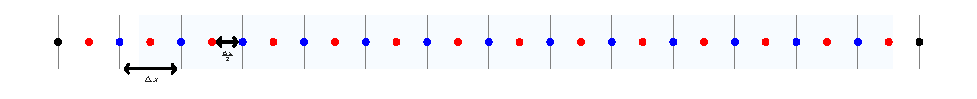
\includegraphics[width=0.8\paperwidth]{staggered}
	\caption{1D Staggered grid.}
\end{figure}

\begin{equation*}
	D^{\left(2\right)}=
	\frac{1}{h}
	\begin{bNiceMatrix}
		1 & 0 & 0 \\
		0 & 1 & 0 \\
		0 & 0 & 1
	\end{bNiceMatrix}.
\end{equation*}

\begin{equation*}
	A=
	\begin{bNiceMatrix}
		a_{11} & \cdots & a_{1c} \\
		\vdots & \ddots & \vdots \\
		a_{r1} & \cdots & a_{rc}
	\end{bNiceMatrix},
	B=
	\begin{bNiceMatrix}
		b_{11} & \cdots & b_{1q} \\
		\vdots & \ddots & \vdots \\
		b_{p1} & \cdots & a_{pq}
	\end{bNiceMatrix}
	A\otimes B\coloneqq
	\begin{bNiceMatrix}
		a_{11}B & \cdots & a_{1c}B \\
		\vdots  & \ddots & \vdots  \\
		a_{r1}B & \cdots & a_{rc}B
	\end{bNiceMatrix}.
\end{equation*}

\begin{equation*}
	D^{\left(k\right)}_{xy}=
	\begin{bNiceMatrix}
		\widehat{I}_{n}\otimes D^{\left(k\right)}_{x} &
		D^{\left(k\right)}_{y}\otimes \widehat{I}_{m}
	\end{bNiceMatrix}.
\end{equation*}

\begin{equation*}
	D^{\left(k\right)}_{xyz}=
	\begin{bNiceMatrix}
		\widehat{I}_{o}\otimes
		\widehat{I}_{n}\otimes
		D^{\left(k\right)}_{x} &
		\widehat{I}_{o}\otimes
		D^{\left(k\right)}_{y}\otimes
		\widehat{I}_{m}        &
		D^{\left(k\right)}_{z}\otimes
		\widehat{I}_{n}\otimes
		\widehat{I}_{m}        &
	\end{bNiceMatrix}.
\end{equation*}

\begin{equation*}
	G^{\left(k\right)}_{xy}=
	\begin{bNiceMatrix}
		\widehat{I}^{T}_{n}\otimes
		G^{\left(k\right)}_{x} \\
		G^{\left(k\right)}_{y}\otimes
		\widehat{I}^{T}_{m}
	\end{bNiceMatrix}.
\end{equation*}

\begin{equation*}
	G^{\left(k\right)}_{xyz}=
	\begin{bNiceMatrix}
		\widehat{I}^{T}_{o}\otimes
		\widehat{I}^{T}_{n}\otimes
		G^{\left(k\right)}_{x} \\
		\widehat{I}^{T}_{o}\otimes
		G^{\left(k\right)}_{y}\otimes
		\widehat{I}^{T}_{m}    \\
		G^{\left(k\right)}_{z}\otimes
		\widehat{I}^{T}_{n}\otimes
		\widehat{I}^{T}_{m}
	\end{bNiceMatrix}.
\end{equation*}

\begin{align*}
	D & =DR. \\
	G & =LG  \\
\end{align*}
